% Chapter 1

\chapter{Resultados} % Main chapter title

\label{Cap_Res} % For referencing the chapter elsewhere, use \ref{Chapter1} 

----------------------------------------------------------------------------

En los dos experimentos realizados, los patrones de respuesta identificados como parte del Efecto Espejo, tanto en la emisión de juicios binarios de detección como en la escala de confianza, se encontraron en más de tres cuartas partes de los participantes. De los 20 participantes en el Experimento 1, 17 mostraron evidencia del efecto espejo en la emisión de juicios de detección y 18 en términos de escalas de confianza; en el caso del Experimento 2, 19 de los 21 participantes mostraron evidencia del Efecto Espejo en ambas tareas.\\


We had 20 and 21 participants on Experiments 1 and 2 respectively. In both cases, we found evidence for the Mirror Effect in at least 85\% of the participants. In Experiment 1, we had 17 cases showing the Mirror Effect pattern within the hit and false alarm rates and 18 in terms of Confidence Ratings. In Experiment 2 we had 19 participants showing the Mirror Effect in both patterns of response. All these proportions were statistically significant when we apply a simple Binomial Test (p=0.0025 and p=0.0004, for Experiment 1, and p=0.0002 for Experiment 2).\\

El análisis de datos está organizado en torno a las siguientes puntos:\\

\begin{itemize}
\item Verificar que las condiciones de dificultad son de hecho diferentes.
\item Comparar las tasas de Hits y Falsas Alarmas sean diferentes entre condiciones.
\item Comparar el puntaje de confianza promedio asignado a cada tipo de ensayo entre las condiciones.
\end{itemize}

Cada uno de estos puntos será abordado desde dos enfoques:\\

\begin{itemize}
\item La réplica de lo reportado en la literatura.

Considerando que el objetivo principal de la investigación aquí desarrollada fue probar la generabilidad de los patrones de respuesta identificados como Efecto Espejo dentro del estudio de la Memoria de Reconocimiento, se

\item El desarrollo de modelos Bayesianos para la éstimación paramétrica.



\end{itemize}

\section{Las condiciones de dificultad son diferentes}

Las condiciones de dificultad propuestas para los experimentos realizados, se construyeron con base en los hallazgos reportados por \parencite{Masaro1971} en cuanto al efecto que tienen las diversas variables que componen las figuras de Ebbinghaus. De acuerdo con estos autores, una de las variables cuyo impacto en la intensidad de la ilusión de Ebbinghaus es más claro, es el número de círculos que aparecen en torno al círculo central.



\begin{figure}[th]
\centering
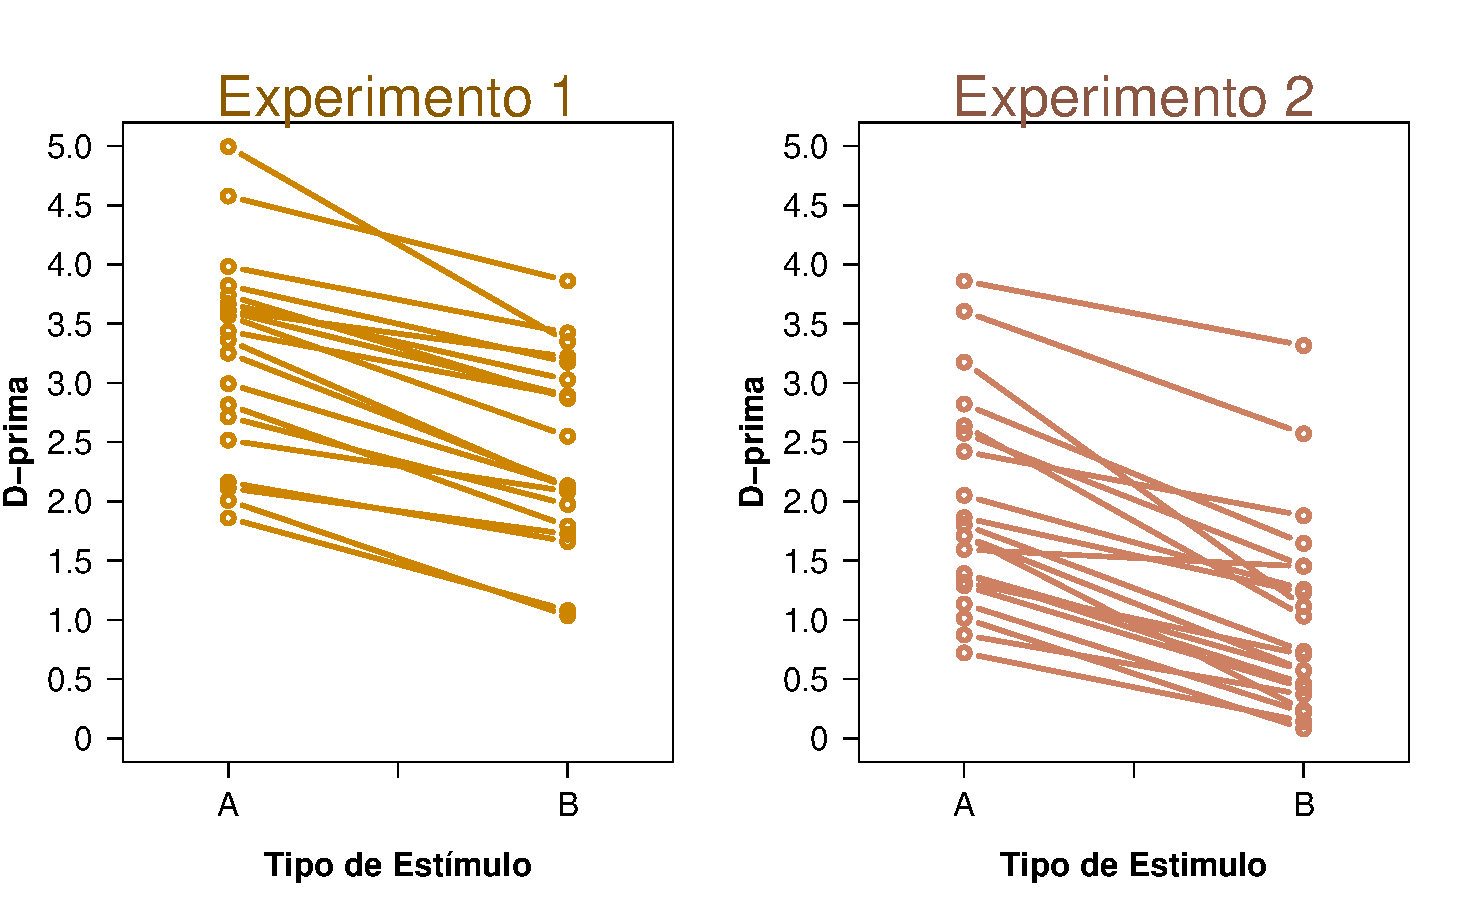
\includegraphics[width=0.80\textwidth]{Figures/Diff_D_E1yE2}
%\decoRule
\caption[Diferencias en Discriminabilidad (Comprobando diferencias entre condiciones)]{ }
\label{fig:Diff_D}
\end{figure}

%----------------------------------------------------------------------------------------

\section{Diferencias en las Tasas de Hits y Falsas Alarmas}

\begin{figure}[th]
\centering
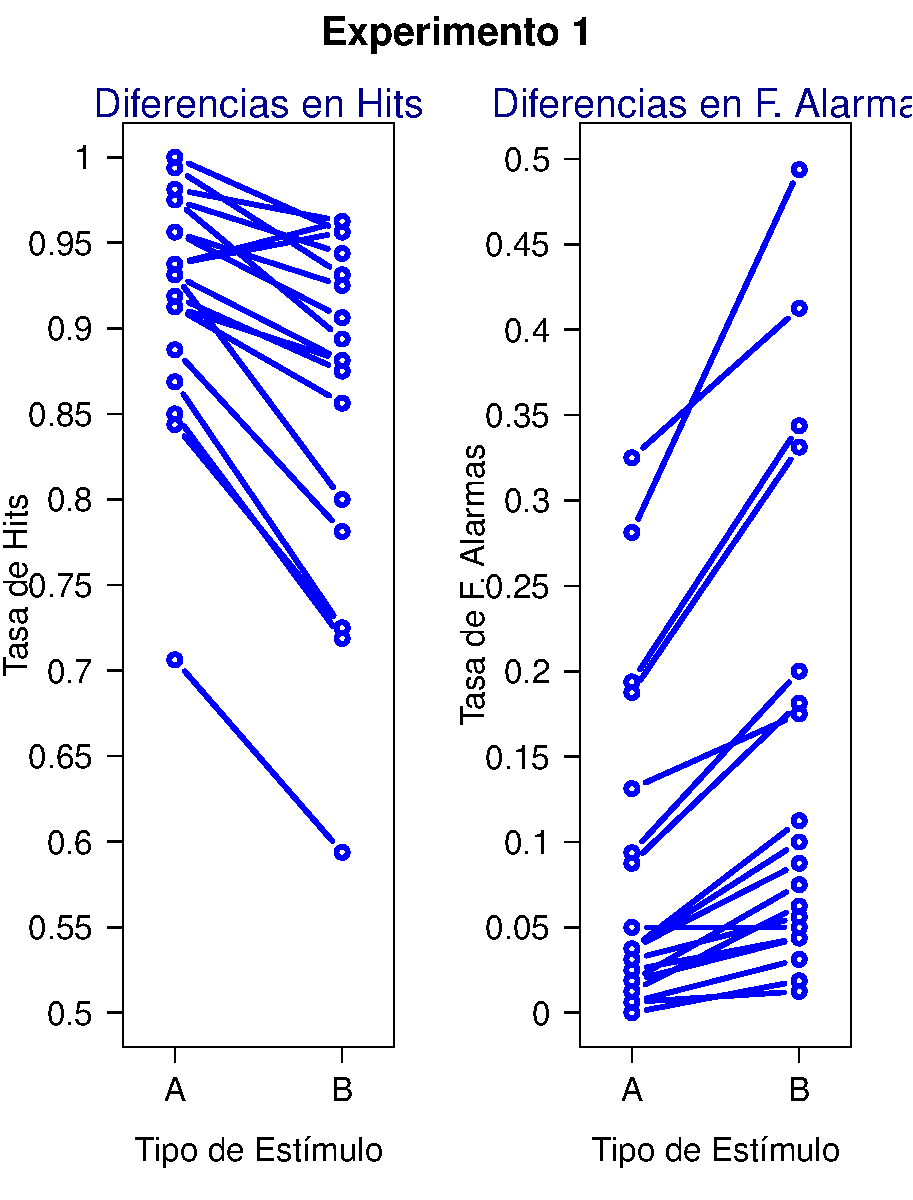
\includegraphics[width=0.80\textwidth]{Figures/Diff_Rate_E1}\\ 
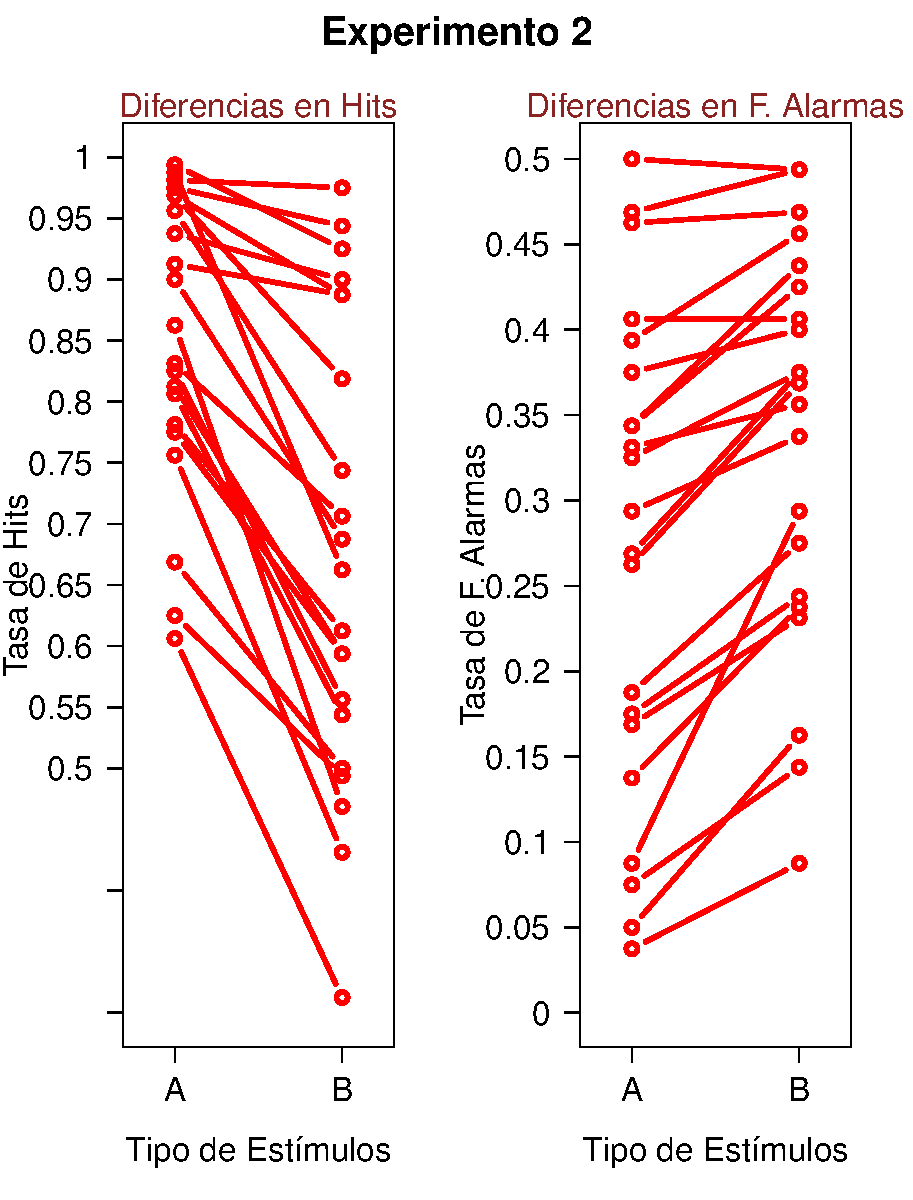
\includegraphics[width=0.80\textwidth]{Figures/Diff_Rate_E2}
%\decoRule
\caption[Diferencias en Tasas (Comprobando diferencias entre condiciones)]{Comparación intrasujeto de}
\label{fig:Diff_Rate}
\end{figure}

\section{Diferencias en la asignación de Puntajes de Confianza}



